\documentclass[a4paper,12pt]{article}
\usepackage[margin=2cm]{geometry}
\usepackage[hidelinks]{hyperref}
\usepackage{graphicx}
\usepackage{float}
\usepackage{enumerate}
\usepackage{amsmath, amssymb}
\usepackage{mathtools}
\usepackage[utf8]{inputenc}
\usepackage{url}
\usepackage[nottoc,numbib]{tocbibind}

\setlength\parindent{0pt}
\pagestyle{empty}
\numberwithin{equation}{section}



% DRM macros
\newcommand{\drm}{\text{DRM}}
\newcommand{\nodrm}{\overline{\drm}}

% Whole game payoff macros (game_number, player number).
\newcommand{\artistpayoff}[2]{\pi_{#1, M_{#2}}}
\newcommand{\firmpayoff}[2]{\pi_{{#1}, F_{#2}}}

% Part game payoff macros.
\newcommand{\artistalbum}[2]{\pi_{#1, M_{#2}, A}}
\newcommand{\artistticket}[2]{\pi_{#1, M_{#2}, T}}
\newcommand{\firmalbum}[2]{\pi_{#1, F_{#2}, A}}
\newcommand{\firmticket}[2]{\pi_{#1, F_{#2}, T}}

% Derivative macros.
\newcommand{\deriv}[2]{\frac{d #1}{d #2}}
\newcommand{\doublederiv}[2]{\frac{d^2 #1}{d {#2}^2}}

% DRM influence on album demand.
\newcommand{\drminf}{(\psi \epsilon - \gamma)}

% Ceiling commands.
\def\lc{\left\lceil}   
\def\rc{\right\rceil}

\begin{document}

% Title Page.
\begin{titlepage}
\begin{center}

\vspace*{5cm}
\Large
\textbf{Game Theory, DRM, Music and Video Games}

\vspace*{0.5cm}
\large
\textsc{Hugo Lhuillier}\\
Sciences Po\\[1.2em]
\textsc{Mitch Mastroni}\\
University of California, Santa Cruz\\[1.2em]
\textsc{Boonrith Pongrasamiroj}\\
Thammasat University\\[1.2em]
\textsc{Michael Sproul}\\
University of Sydney

\vspace*{3cm}
\textsc{Group 2}\\[1.2em]
\textsc{ECON 166A, Fall 2014}\\
University of California, Santa Cruz

\vfill

\today

\end{center}
\end{titlepage}
\pagebreak

\section{Introduction}

\section{Literature Review}

We begin with the paper that is interesting but yet simple called ``The DRM Game'' by Heileman G et al \cite{heileman2007}. It shows the game theoretical analysis of DRM as a simple extensive form game as well as a more advance strategic form game. The first analysis consists of vendor and consumer playing a sequential move one-shot game where the consumer moves first. The consumer is, then, required to take an action on whether to purchase or illegally download. Vendor has an option to implement technological protection or not. The paper further shows that DRM could not be perfect, as in there will definitely be some leak even with the presence of technological protection thus allows file sharing to happen even in the case of DRM. More importantly, they focus on its subgame where, after both players choose the actions mentioned above, consumer decides to share or not to share files he or she obtains and vendor chooses whether to take a legal action against the consumer or not. The game needs to be solved with mixed strategy Nash equilibrium with the probability that vendor will take an action as low as around 0.4\% of the time. An important aspect that this paper gives us an insight about is that DRM is a negotiating game. In a repeated game where consumer and vendor play this game repetitively, the outcome is the same as a one-shot game. The equilibrium of this game has to be mixed. Both parties negotiate, indirectly through the repetitive nature of the game, until it is such that consumer’s behavior drives vendor to take an action against them meanwhile vendor’s action will force consumer to stop sharing. Hence, they conclude that the in the repeated game the equilibrium would be such that no matter the vendor imposes technological protection or not, the consumer will not share the content and the vendor will take action against piracy, even though they rarely do so.\\

In ``Who should own access rights? A game-theoretical approach to striking the optimal balance in the debate over Digital Rights Management'' by Yu-Lin Chang \cite{chang2007}, he approaches the problem in a very interesting way. The problem could not be solved by only looking at one aspect, namely, economics but need to be approached carefully on various sides. Chang introduces the concept of ``the notation of balance'' and argues that the way to solve this problem of implementing DRM is neither to give full restriction to the firm nor totally free access of the content to the public. He claims that it is about the right balance of the rights distributed between the two parties. While DRM in the past tended to limit the use of users who purchased the content, it fails miserably. At the same time, the era of free access when internet spread worldwide caused the information industry to lose a lot of money and was in trouble. The Nash equilibrium is when there is a correct amount of balance between the consumer’s right and the firm’s right to access to the content. Chang offers the solution that happens to be a prisoner’s dilemma where the Nash equilibrium is better for the society as a whole but is not the best for each player in the game.\\

There also is a paper which applies mathematics and computer programming to the analysis of how DRM works. Zhang, Pei, Ma, and Yang show in their paper ``Game-Theoretic Analyses and Simulations of Adoptions of Security Policies for DRM in Contents Sharing Scenario'' \cite{zhang2011} the method of constructing a payoff equation and matrices for provider and sharer. The game is shown as a simultaneous-move game. Later on, the game is evolved to dynamic and mixed game with two players, providers and sharers. They later on develop a simulation that simulates the repeated game with many sharers and providers as in the case of reality. The equilibrium occurs when the game is at all-enhanced security strategy. That is providers will forfeit all-general security, the old method of DRM which encrypt the files and make it very inconvenient to use in general, and turn to all-enhanced security strategy. They explain that it is a new method of DRM with higher security that enables users to share the content within their trusted devices, hence allows them to use the content as their wills within the acceptable constraint agreed by both providers and sharers.

\section{Model}
\subsection{Game Setting}

The DRM game is made of two categories of player, the record labels and the artists. The record labels are, with the artist, the major actors of the music industry market; indeed, a record label is a publishing company which ``coordinates the production, manufacture, distribution, marketing, promotion, and enforcement of copyright for sound recordings and music videos''\cite{klein2014}. Interestingly for this game is to note that there are a limited numbers of record labels in the current music industry market. According to the 2005 IFPI report, four firms were controlling more than three-fourth of the market in 2005; specifically, Universal Music Group had 28.8\% of the market, Sony Music Entertainment 21.1\%, EMI 14.1\%, and Warner Music Group 13.4\%.\\

The second category of players is the artist. Note that, even though the game represents the music market industry, consumers are not explicitly considered as players in the game, neither in the underlying model. Nonetheless, as DRM affect consumers' behaviors, either by forcing them to buy album by fighting illegal piracy, or by decreasing their willingness to pay for albums, consumers' preferences are incorporated into firms' and artists' profit function, as presented in the next section.\\

The whole game is divided into two games, with first a pricing game, and then the DRM game properly speaking.\footnote{
This duality is not consistent with the reality; in the real music industry market, firms decide simultaneously whether they want to implement DRM systems, and the price of their albums and concert tickets. However, in order to keep the model simple, we assumed that they were first fighting over the price of their products, and then taking a decision about DRM, maintaining those prices constant.
}\\

In the first game, the first players to move are the firms, competing against each other in order to maximize their profit by varying their album and concert tickets prices. When fixing its prices, a given firm does not know what the other firms are doing. Notice that prices have two effects in this game; first, by fixing higher prices than other record labels, a given firm appears as more profitable for artists. Therefore, more artists are likely to sign a contract with this record label, increasing ultimately its profit. However, higher prices imply in the meantime a lower demand for a given record label, potentially decreasing its profit.\\

Artists, observing prices fixed by record labels, decide then with which firms they want to sign a contract. For simplicity, they cannot quit the market, or be independent.\\

Follow this first game the DRM game, in which the album and concert ticket prices taken into account by the players are the ones determined in the first game. In this new game, firms choose first whether they want to enforce DRM systems in their product. A record label cannot decide to implement DRM only for some artists.  Enforcing DRM systems can have two opposite effects on a firm's profit. On one hand, by decreasing the number of illegal download, DRM increases the demand for album. On the other hand, consumers can have an aversion for album with DRM inside, triggering a decrease in the album demand. Moreover, artists can also dislike DRM since it could potentially decreases the exposure of their work, and, ergo, the number of people going to their concerts. The effect of DRM on firms' and artists' profit depends therefore on the relative impact of these two effects.

% EFG figure.
\begin{figure}[h]
\centering
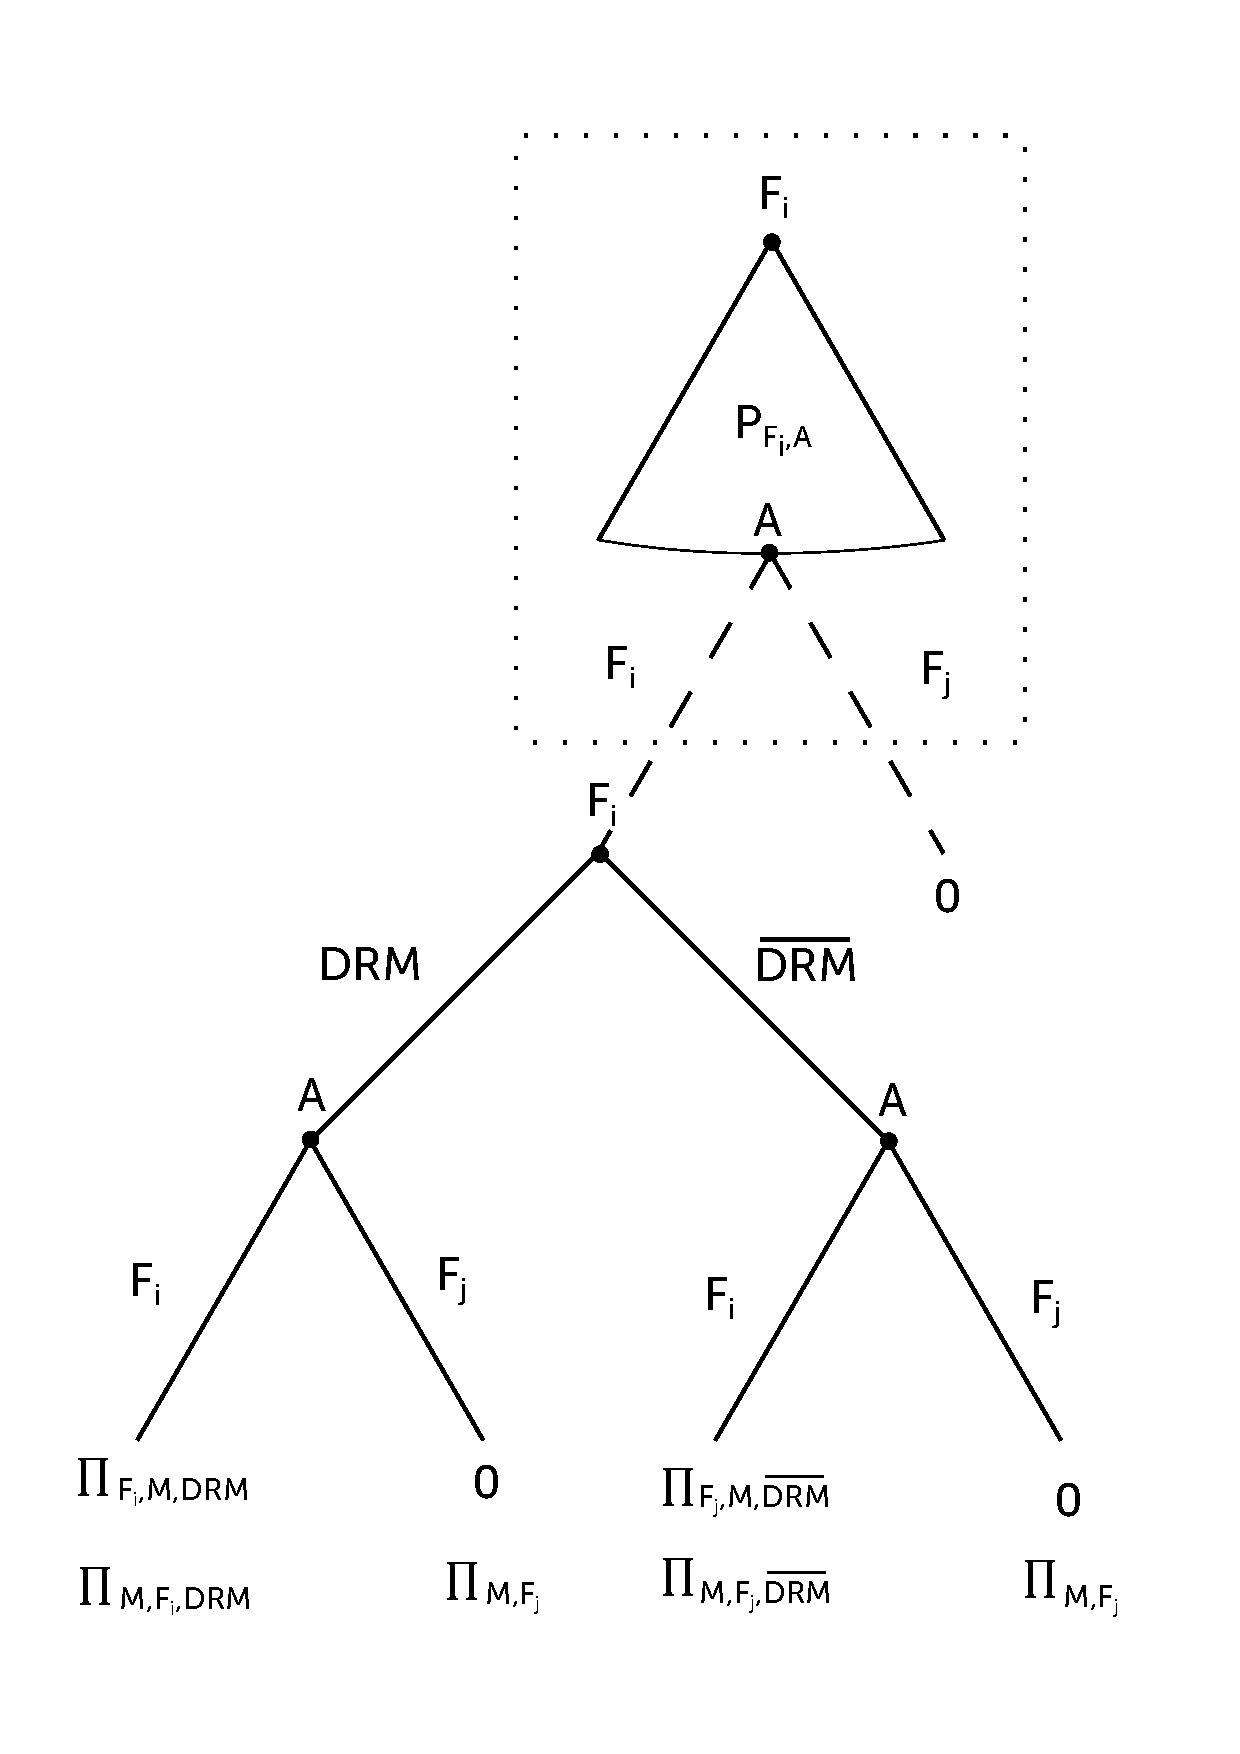
\includegraphics[width=12cm]{Graphics/GameTree.pdf}
\caption{Extensive Form Game for the Whole Game, from a Record Label's Perspective.}
\end{figure}

Figure 1 summarizes the previously described game configuration into an extensive form game. The dash box around the first two nodes represents the separation between the two games. Note that, for simplicity purpose, this figure is not the entire extensive form game, but the description of the game from a record label's point of view. Specifically, after deciding of a price, $P_{A, F_i}$, the artist can decide whether to go with this given record label, $F_i$, or any other firms, $F_j$, $i \ne j$. In the second game, the same label chooses whether enforcing DRM systems in its products, and the artist, once more, decides if he or she wants to go with this firm. If the artist opts for another firm, $F_j$, $F_i$'s profit is zero. If, on the contrary, the artist selects $F_i$, $F_i$'s payoff is positive, as described in the following section.

\subsection{Payoff Functions}

\subsubsection{Game 1: Pricing Game}

Firms are profit maximizer, that being true even in the music industry. Firms' payoff can therefore be described by a profit function such as $\pi_{F_i} = TR_{F_i} - TC_{F_i}$.\\

The record labels' revenues are made of the sales from the artists' albums under their label, tours and concerts from those same artists, and merchandising. For simplicity purpose, merchandising revenues are assumed to be constant for the four firms, so that firms' profits ultimately rely on revenues from album sales \& concerts \footnote{
A more realistic assumption is that merchandising revenues are a function of the albums and tickets sales – the more famous an artist is, the more album he or she sold, as well as tickets, the more merchandise products his or her fans purchase. In both case, record labels will try to maximize the quantity of albums and tickets sold to maximize the quantity of merchandise products.
}.\\

On the other side, record labels' costs are composed for more than two third of their total costs of marketing \& promotion expenditures, selling, general \& administrative expenses, and royalty payments. Because marketing \& promotion are not the topics of interest of this paper, they are assumed to be constant for the four firms, and, ergo, not taking into consideration into the model. Record labels' costs can be reduced to the payments of the artists under their label.\\

Therefore, the profit of a given firm, $F_i$, for a particular artist (musician) within the record label, $M$, can be describe as:
\begin{eqnarray}
\pi_{F_i, M} = \pi_{F_i, M, A} + \pi_{F_i, M, T}
\label{Eq:FirmTotalPayoff}
\end{eqnarray}  

Where $\pi_{Fi, M, A}$ is the record label's profit depending on the quantity of album sold for an artist $M$, and $\pi_{F_i, M, T}$ the record label's profit varying in function of the number of concert tickets sold for the same artist $M$. Specifically:
\begin{eqnarray}
\pi_{F_i, M, A} = (a_{A, M} - \sigma_{A, M} P_{A, M})(1 - \alpha_{A, M}) P_{A, M}
\label{Eq:FirmAlbumPayoff}
\end{eqnarray}

With $a_{A, M}$ a constant standing for the demand for the album of a given artist when its price is zero, $\sigma_{A, M}$ a constant expressing the variation of album sold induced by a marginal variation in album price, $P_{A, M}$ the price of an album $A$ for an artist $M$, fixed by the record label $F_i$, $a_{A, M}, \sigma_{A, M}, P_{A, M} > 0$, and $\alpha_{A, M}$ the album sharing rules determined by the record labels, $0 < \alpha_i < 1$. Equation $\eqref{Eq:FirmAlbumPayoff}$ is nothing more than a usual profit function, where the left-side of the equation represents the demand for albums - the demand being negatively related to the album price, and the right side of the equation describes the profit per album, namely the difference between the price of the album and its costs, assumed to be only made of the part of the price the record label is ready to giving up to the artist.\\

Similarly for the concert tickets profit:
\begin{eqnarray}
\pi_{F_i, M, T} = (a_{M, T} - \sigma_{M, T} P_{M, T})(1 - \alpha_{M, T}) P_{M, T}
\label{Eq:FirmTicketPayoff}
\end{eqnarray}

$a_{M, T}$ is a constant portraying the demand for concert tickets of a given artist when its price is zero, $\sigma_{M, T}$ is a constant precising the variation of concert ticket sold triggered by a marginal variation in concert ticket price, $P_{M, T}$ is the price of a concert ticket, $a_{M, T}, \sigma_{M, T}, P_{M, T} > 0$, and $\alpha_{M, T}$ the concert ticket sharing rules, also determined by the record labels, $0 < \alpha_i < 1$.\\

Substituting \eqref{Eq:FirmAlbumPayoff} and \eqref{Eq:FirmTicketPayoff} into \eqref{Eq:FirmTotalPayoff} yields the following record label’s profit function for one of its artists, $M$:
\begin{eqnarray}
\pi_{F_i, M} = (a_{M, A} - \sigma_{M, A} P_{M, A})(1 - \alpha_{M, A}) P_{M, A} +
	(a_{M, T} - \sigma_{M, T} P_{M, T})(1 - \alpha_{M, T}) P_{M, T}
\end{eqnarray}

To simplify this model, the albums and concert tickets prices are presumed equal for all artists within a record label, as well as the album and concert tickets sharing rules \footnote{
These assumptions are empirically not true; however, this paper is interested in looking at how competition between firms shapes the decisions about whether or not implementing DRM systems. In that sense, even though prices are obviously different among artists within a record label, one can consider $P_{M, A}$ and $P_{M, T}$ as the mean of all different possible prices of albums and concert tickets within a record label. The same explanation can be provided for $\alpha_A$ and $\alpha_T$ equal for all artists within a firm.
}.

Moreover, it is assumed that the album and tickets demand when the price is zero, the price elasticity of album and concert tickets, and the album and concerts sharing rules are equal for the four labels, such that $a_{M, A} = a_A$. Additionally, the concert ticket price can be expressed as a function of the album price:
\begin{eqnarray*}
P_{i, T} = k P_{i, A}
\end{eqnarray*}

Where $k$ is a constant defined as the average concert ticket price over the average album price, $k > 0$. Adding altogether those changes shows the following record label’s profit function for a given artist, $M$:
\begin{eqnarray}
\pi_{F_i, M} = (a_A - \sigma_A P_{F_i, A})(1 - \alpha_A) P_{F_i, A} +
	(a_T - \sigma_T k P_{F_i, A}) (1 - \alpha_T) k P_{F_i, A}
\end{eqnarray}

From here, record label’s profit function for any artist being the same for all artists under contract with it, its total profit function is the sum of the per artist profit:
\begin{eqnarray}
\pi_{F_i} = l_{F_i} (a_A - \sigma P_{F_i, A})(1 - \alpha_A) P_{F_i, A} +
	(a_T - \sigma_T k P_{F_i, A})(1 - \alpha_T) k P_{F_i, A}
\end{eqnarray}

$l_{F_i}$ standing for the number of artist under contract with the record label, $l_{F_i} \in [0, n]$, such that $\sum_{i = 1}^m l_i = n$, $n$ being the total number of artists in the music industry market, $m$ being the number of firms (in our case, 4).\\

The other players’ payoffs, namely the artists’ payoffs, are defined similarly. Specifically, their album and concert demands are the same as the record labels’ ones, and their profit per unit are the complement of the record label’s revenue, i.e. the share of the concert ticket or album price the record label accept to give to them, $\alpha P_{F_i, A}$ or $\alpha_T k P_{F_i, A}$. Eventually, making an album or putting on a concert is not without costs to the artist, so the constants $C_A$ and $C_T$, where $C_A, C_T > 0$,  encode the cost of producing an album and a concert series respectively. Those two finals parameters are assumed to be fixed cost defined exogenously\footnote{
This assumption is consistent with the reality of the music market industry since, most of the time, artists sign a contract with a record label stipulating a priori how much the production of an album will cost to them, and this cost does not evolve with the number of album sold.
}. Formally, the payoff function of a given artist, $M$, is given by:
\begin{eqnarray}
\pi_M = (a_A - \sigma_A P_{F_i, A})\alpha_A P_{F_i, A} - C_A
	+ (\alpha_T - \sigma_T k P_{F_i, A}) \alpha_T k P_{F_i, A} - C_T
\end{eqnarray}

This formal description of the model is useful to define the player’s strategy set. The four firms, $F_i$, playing first, chooses $P_{F_i, A} > 0$, followed by the artists, signing a contract with a record label $F_i, i \in [0, m], where m = 4$. Because all artists have the same payoff function, a representative artist is designated as the only player for the artist category. 

\subsubsection{Game 2: DRM Game}

The second game studies whether record labels have incentives to implement DRM in their products. The players’ payoff functions are mainly based on the same framework as the first game, except that $P_{F_i, A}$ is now considered as a constant, and no longer as an independent variable.\\

Formally, recalling that a firm’s album and a firm’s ticket concert profit are:
\begin{eqnarray}
\pi_{F_i, A} = l_{F_i} (a_A - \sigma_A P_{F_i, A})(1 - \alpha_{F_i, A}) P_{F_i, A}\\
\pi_{F_i, T} = l_{F_i} (a_A - \sigma_A P_{F_i, A})(1 - \alpha_{F_i, T}) k P_{F_i, A}
\end{eqnarray}

The new payoff function is defined as:

\begin{eqnarray}
\firmpayoff{2}{i} = \firmalbum{1}{i} (D_A) + \firmticket{1}{i}  (D_T) - C_{\drm}
\label{Eq:FirmTotalPayoffDRM}
\end{eqnarray}

Where $D_A$ and $D_T$ are respectively the impact of DRM on the album and ticket concert profit, and $C_{\drm}$ stands for the cost of implementing DRM systems. Specifically:
\begin{eqnarray}
D_A = 1 + \delta \drminf
\label{Eq:DA}
\end{eqnarray}

With $\delta$ a binary variable, $\delta \in \{0, 1\}$, equal to one when DRM systems are enforced, $\psi$ the number of illegal download for a record label, and $\gamma$ the consumers’ disutility of purchasing an album with DRM in it, $\psi > 0, \gamma \geq 0$. DRM can indeed be viewed as a constraint from the consumer’s point of view, reducing his or her willingness to pay for a given album. Eventually, $\epsilon$ represents the effectiveness of DRM to fight illegal piracy, $0 \leq \epsilon \leq 1$, such that if $\epsilon = 1$, DRM systems are extremely effective and illegal download no longer exists. Therefore, $\drminf$ describes the tradeoff record labels are facing when they are deciding whether they should implement DRM systems.\\

Similarly:
\begin{eqnarray}
D_T = 1 - \delta \theta
\label{Eq:DT}
\end{eqnarray}

Where $\theta$ is the number of tickets non-sold due to the presence of DRM on firms’ products, coming both from the fact that consumers do not want to go to concerts of artist who have DRM on their music and from the fact that the music of artists with DRM systems can be less spread due to more difficulties to illegally download the product, generating therefore less fans, $\theta > 0$.\\

Eventually, implementing DRM systems has a cost:
\begin{eqnarray}
C_\drm = \frac{\rho}{l_{F_i} + 1}
\label{Eq:CostDRM}
\end{eqnarray}

$\rho$ portraying the cost of DRM, $\rho > 0$. Implicit in this cost function is that economies of scale exist, such that, for a given value of $\rho$ for a given firm, the cost of implementing DRM will decrease as the number of artists within this label increases.\\

Equation \eqref{Eq:FirmTotalPayoffDRM} can be seen in terms of percentage. If a firm decides to not implement DRM, then delta equals zero, and its payoff, $\firmpayoff{2}{i}$, is identical to the one derived in the previous game (100\%). If, on the contrary, a record label chooses to go for DRM, then its profit evolves by $\drminf$, depending on the effectiveness of DRM and the way consumers dislike DRM, $\drminf$ defining a percentage of the previous profit, possibly greater or smaller than 100\%\footnote {
Section \ref{Sec:Estimates} estimates those parameters and substitutes them into the profit functions, which can help to better understand the new payoff function if this is not already the case.
}.\\

In order to not add further complexity to this model, $\gamma$, $\psi$ and $\epsilon$ are assumed to be constant and equal for all firms. Of particular interest for our topic, $\epsilon$ is defined exogenously, such that record labels have no control over the effectiveness of DRM. This strong assumption is discussed in section \ref{Sec:Extensions}, where possible extensions of the model are presented.\\

Substituting \eqref{Eq:DA}, \eqref{Eq:DT} and \eqref{Eq:CostDRM} into \eqref{Eq:FirmTotalPayoffDRM} yields:
\begin{eqnarray}
\firmpayoff{2}{i} = l_{F_i} \left[
	(1 + \delta \drminf) \firmalbum{1}{i} +
	(1 - \delta \theta) \firmticket{1}{i}
\right]
- \delta \left( \frac{\rho}{l_{F_i} + 1} \right)
\end{eqnarray}

Regarding the representative artist’s payoff, the impact of DRM on his or her profit is the same as the one for the record labels. Formally, his or her new payoff function is given by:

\begin{eqnarray}
\artistpayoff{2}{i} = (1 + \delta \drminf) \artistalbum{1}{i} - C_A +
						(1 - \delta \theta) \artistticket{1}{i} - C_T
\end{eqnarray}

Once more, this formal description is useful to derive players’ strategy set. Firms, acting first, choose $\delta \in \{0, 1\}$, followed by the representative artist, deciding to sign a contract with one of the four labels, $F_i$, $F_i \in \{F_1, F_2, F_3, F_4\}$.

\pagebreak
\section{Solutions}

\subsection{Game 1: Pricing Game}

To solve the pricing game, we considered the optimal price desired by the artists. All the artists have the same payoff function, $\artistpayoff{1}{i}$, which depends on the continuous variable $P_A$ and no discretely valued variables. Therefore it is possible to maximise $\artistpayoff{1}{i}$ using simple calculus. Given an artist-optimal value of the album price, $P_A^*$, we prove that the firms must all set this price in any Nash Equilibrium utilising pure strategies.\\

Imagine a situation where the firms have agreed on prices such that the highest price chosen by a firm is $P_A^- < P_A^*$. In this case, all firms not already choosing $P_A^-$ have a best response to increase their price to $P_A^-$ in order to make them indistinguishable from the top firm(s), which would otherwise take the business of all the artists. Artists care only about getting as close to $P_A^*$ as possible, and will always choose the firm that offers the closest price. To this end, the firms all have a best response to increase their price to get closest to $P_A^*$. With this pressure applied from the upwards direction as well, it's clear that the only equilibria will have all of the firms setting their price at $P_A^*$.\\

With all the firms offering the same price, the artists have no way to distunguish them, and can choose arbitrarily without destroying the equilibria. Given that each of the $n$ artists has a choice of $m$ firms, this gives rise to $m^n$ Nash Equilibria in the pricing game.\\

$P_A^*$ can be found by maximising $\artistpayoff{1}{i}$:
\begin{eqnarray*}
\artistpayoff{1}{i} & = & (a_A - \sigma_A P_A)\alpha_A P_A + (a_T - k \sigma_T P_A) k \alpha_T P_A\\
\deriv{\pi}{P_A} & = & a_A \alpha_A - 2 \alpha_A \sigma_A P_A + k a_T \alpha_T - 2 \alpha_T \sigma_T k P_A\\
\doublederiv{\pi}{P_A} & = & -2(\alpha_A \sigma_A + \alpha_T \sigma_T) < 0 \Rightarrow \text{maximum}
\end{eqnarray*}

Solving $\deriv{\pi}{P_A} = 0$ yields:
\begin{eqnarray}
P_A^* = \frac{\alpha_A a_A + k \alpha_T a_T}{2(\alpha_A \sigma_A + k \alpha_T \sigma_T)}
\end{eqnarray}

\subsection{Game 2: DRM Game}

The solution to the DRM game has a similar structure to that of the pricing game. Once again, the artists control the behaviour of the firms, and are free to choose between them. The difference is that the DRM game is paramaterised by a number of constants: $\psi$, $\epsilon$, $\gamma$ and $\rho$, which generate several types of systems. In this section we explore the nature of equilibria in these different systems.\\

Given the payoff function for the artists as follows, note that the artists will have a strict preference for DRM or $\overline{\text{DRM}}$:
\begin{eqnarray*}
\artistpayoff{2}{i} = (1 + \delta (\psi \epsilon - \gamma)) \artistalbum{1}{i} + (1 - \delta \theta) \artistticket{1}{i}
\end{eqnarray*}

This follows from the fact that the payoff from the first game is fixed, and that $\delta$ is a binary variable. Comparing the payoff with DRM to the payoff without, there are three possiblities: either DRM is favourable, $\nodrm$ is favourable, or the payoffs are equal, in which case the artists are ambivalent.\\

First consider the two cases where the payoffs are different. In these cases, the best response of the firms is to set $\delta$ according to the artists' preference. It is impossible to have an equilibrium where the firms set $\delta$ against the artists' preference, as this would result in one firm deviating and stealing the entire market. Hence the only possible equilibria involve all the firms setting $\delta$ in the way that is optimal for the artists. As before, the artists then have no way to differentiate the firms and can choose between them freely, for a total of $m^n$ Nash Equilibria in pure strategies.\\

This isn't quite the whole story however, as the firms also pay a cost for implementing DRM, and may be forced to disable DRM if this cost is prohibitive. Accumulating more artists reduces the cost of DRM, and hence for each system, there is a number of players $\eta$, such that firms with $\eta$ or more players are better off if they implement DRM. Computing the value of $\eta$ is done by equating the two firm payoffs:
\begin{eqnarray*}
\firmpayoff{2}{i}(\delta = 1, l_i = \eta) & = & \firmpayoff{2}{i}(\delta = 0, l_i = \eta)\\
\eta \left[\left(1 + \delta \drminf\right) \firmalbum{1}{i} + (1 - \delta \theta) \firmticket{1}{i}\right] - \frac{\rho}{\eta + 1} & = & \eta (\firmalbum{1}{i} + \firmticket{1}{i})
\end{eqnarray*}

Solving for (positive) $\eta$ yields:
\begin{eqnarray}
\eta & = & \lc \frac{-1 + \sqrt{1 + 4 x}}{2} \rc \\
\text{where } x & = & \frac{\rho}{\drminf \firmalbum{1}{i} - \theta \firmticket{1}{i}} \nonumber
\end{eqnarray}

We are now in a position to classify some more system behaviour. If $\eta = 1$, then it is always beneficial for firms to implement DRM, given a fixed value of $l_i > 0$. We say that the DRM is \textit{strongly firm-beneficial}. At the other extreme, if $\eta > n$, then firms are worse-off implementing DRM for a fixed choice of $l_i > 0$, and we say that the DRM is \textit{strongly firm-detrimental}. Note that the presence of strongly beneficial or strongly detrimental DRM is not sufficient to predict what the firms will choose, due to the market effect introduced by the artists. As explained above, if artists prefer one DRM state to another, firms must choose that state to avoid losing the entire market. The exception to this is firms with no artists, which must always choose $\nodrm$, to avoid a negative payoff. The resulting dynamics are best captured by an exhaustive enumeration of possible scenarios.
\begin{itemize}
\item Artists prefer DRM.
	\begin{itemize}
	\item DRM is strongly firm-beneficial ($\eta = 1$): All firms with associated artists enable DRM. Any configuration of this form is a Nash Equilibrium.
	\item DRM is strongly firm-detrimental ($\eta > n$): As long as the firm payoff for implementing DRM is not negative, all equilibria involve firms with non-zero $l_i$ enabling DRM due to the market effect, and firms with $l_i = 0$ disabling DRM to avoid negative payoffs. If the firm payoff is negative for values of $l_i > l_i^* > 0$, then the system is \textit{degenerate}. In the interests of brevity we don't consider such systems here.
	\item DRM is firm-moderate ($1 < \eta \leq n$): Nash Equilibria in this case are comprised of some firms with DRM enabled and $l_i \geq \eta$, and others with DRM disabled and $l_i = 0$.
	\end{itemize}
\item Artists prefer no DRM.\\
In this case, the firm preference is irrelevant. At equilibrium, all firms disable DRM and artists associate freely.
\end{itemize}

In the case where artists are ambivalent to DRM, equilibria are characterised by some firms with DRM enabled and $l_i \geq \eta$, and others with DRM disabled and $\eta < \eta$. This is similar to the case where artists prefer DRM and DRM is firm-moderate, except that firms without DRM can posess artists at equilibrium.\\

Finally, we come to describing the parametrisations that cause artists to prefer one DRM state over another. It would take many pages to quantify the influence of all three parameters influencing artists ($\psi, \epsilon$, $\gamma$ and $\theta$), so we concern ourselves only with $\epsilon$ - the effectiveness of DRM in preventing piracy - as it is the least well known. In the next section we provide real-world estimates of the other parameters.\\

To compute the critical value of $\epsilon$ at which artist preferences flip, we solved the following inequation involving the payoffs with and without DRM:
\begin{eqnarray*}
\artistpayoff{2}{i}(\delta = 1) & > & \artistpayoff{2}{i}(\delta = 0)\\
(1 + \delta \drminf) \artistalbum{1}{i} + (1 - \delta \theta) \artistticket{1}{i} & > & \artistalbum{1}{i} + \artistticket{1}{i}
\end{eqnarray*}

Solving for $\epsilon$ we have that DRM is artist-beneficial when:
\begin{eqnarray}
\epsilon > \frac{1}{\psi} \left( \frac{\theta \artistticket{1}{i}}{\artistalbum{1}{i}} + \gamma \right)
\end{eqnarray}

When $\epsilon$ is equal to the term on the right, which we shall call $\epsilon^*$, the payoffs are equal and the artists are DRM ambivalent. Combined with the characterisations from above, and values for $\psi, \gamma, \theta$ and $\rho$ this allows us to predict the equilibrium behaviour of a DRM system where $\epsilon$ is uncertain.\\

Conceptually, the tension between artists and firms over DRM is a consequence of varying valuations of albums and concerts, and the impact that DRM has on both. Whilst it is possible (and even likely), for DRM to have little impact on concerts, this can have a profound impact on the dynamics of the game if arists receive more of their revenue from concerts ($\alpha_T \gg \alpha_A$), and therefore feel the impact of DRM stronger than the firms. Conversely, firms are more likely to be negatively effected by DRM if $\drminf$ is large, and firms draw most of their revenue from album sales ($\alpha_T \ll \alpha_A$). This interaction is discussed further in section \ref{Sec:Estimates}.

\pagebreak
\section{Estimation of Parameters} \label{Sec:Estimates}

\subsection{Real World Solutions}



\section{Extensions to the Model} \label{Sec:Extensions}

\section{Implications for the Video Game Industry}

\section{Conclusion}

\bibliographystyle{plain}
\bibliography{References}

\end{document}
